\documentclass[10pt,a4paper,landscape]{article}
\usepackage{multicol}
\usepackage{calc}
\usepackage{ifthen}
\usepackage[landscape]{geometry}
\usepackage{amsmath,amsthm,amsfonts,amssymb}
\usepackage{color,graphicx}
\usepackage{hyperref}
\usepackage{listings}
\usepackage{underscore}
\usepackage{todonotes}
\usepackage{mathtools}

% Cheatsheet style
\input{style.tex}

% Shorthand for \bf
\providecommand{\bf}[1]{\ensuremath{\bf{#1}}}
\newcommand{\bbeta}{\boldsymbol\beta}

\pdfinfo{
  /Title (Machine Learning Cheat Sheet)
  /Creator (TeX)
  /Producer (pdfTeX 1.40.0)
  /Author (Dennis Meier, Jakub Sygnowski)
  /Subject (Machine Learning cheatsheet)
  /Keywords (machinelearning, ml, bayes, regression, classification)
}

% -----------------------------------------------------------------------

\begin{document}
\title{Machine Learning Cheat Sheet}

\raggedright
\footnotesize
\sffamily
\begin{multicols*}{4}

% multicol parameters
% These lengths are set only within the two main columns
%\setlength{\columnseprule}{0.25pt}
\setlength{\premulticols}{1pt}
\setlength{\postmulticols}{1pt}
\setlength{\multicolsep}{1pt}
\setlength{\columnsep}{2pt}

\begin{center}
  \Large{\underline{Machine Learning Cheat Sheet}}
\end{center}

% ----------
\section{Regression}
  We have a set of $N$ training examples of dimensionality $D$, e.g:
  
  $x_n = \begin{bmatrix} x_{n1} \quad x_{n2} \quad ... \quad x_{nD} \end{bmatrix}^T $

  We often put the examples into one matrix with extra column of $1$s:

  $ \widetilde{X} = \begin{bmatrix}
    1 \quad x_{11} \quad x_{12} \quad \ldots \quad x_{1D} \\
    \ldots\\
    1 \quad x_{N1} \quad x_{N2} \quad \ldots \quad x_{ND}
  \end{bmatrix}
  $

  (note that $x_n$ are rows, not columns)

  The goal is to predict a $\hat{y}$ given $x$.

  Simple linear regression: $y_n \approx \beta_0 + \beta_1 x_{n1}$

  Multiple dimension linear regression: $y_n \approx f(x^*) := \beta_0 + \beta_1 x^*_{1} + \beta_2 x^*_{2} + ... + \beta_D x^*_{D}$

  \subsection{Linear basis function model}
  $y_n = \beta_0 + \sum_{i=1}^{M} \beta_i \phi_i(\bf{x_n}) =  \bf{\widetilde\phi^T}(\bf{x}^T_n) \boldsymbol\beta$.
  The optimal $\beta$ is given by $\beta = ( \widetilde{\Phi}^T \widetilde{\Phi})^{-1} \widetilde{\Phi}^T y$ where $\widetilde{\Phi}$ is a matrix with N rows and the n-th row is $[1, \phi_1(x_n)^T,  ...,  \phi_M(x_n)^T]$.

  Ridge regression: $\beta_{ridge} = ( \widetilde{\boldsymbol \Phi}^T \widetilde{\boldsymbol\Phi} + \lambda \boldsymbol I)^{-1} \widetilde{\boldsymbol\Phi}^T \boldsymbol y$

  \subsection{Cost functions}
  \begin{colfig}
    \centering
    \includegraphics[width=\linewidth]{images/error-functions.png}
  \end{colfig}

  Cost function / Loss: $\mathcal{L}(\boldsymbol\beta) = \mathcal{L}(\mathcal{D},\boldsymbol\beta)$

  Mean square error (MSE): $\frac{1}{2N} \sum_{n=1}^{N}\left[y_n-f(\bf{x}_i) \right]^2$

  Mean absolute error (MAE): $\frac{1}{2N} \sum_{n=1}^{N}\left | y_n-f(\bf{x}_i) \right |$

  Huber loss: $\mathcal{L}_\delta (a) = \begin{cases}
   \frac{1}{2}{a^2}                   & \text{for } |a| \le \delta, \\
   \delta (|a| - \frac{1}{2}\delta ), & \text{otherwise.}
  \end{cases}$

  Root mean square error (RMSE): $\sqrt{2 * \text{MSE}}$

  Epsilon insensitive (used for SVMs):
  $\mathcal{L}_{\epsilon}(y, \hat{y}) = \begin{cases}
   0                   & \text{if } |y - \hat y| \le \epsilon, \\
   |y - \hat y| - \epsilon, & \text{otherwise.}
  \end{cases}$

% ----------

\todo[inline]{TODO: statistical/computational tradeoff}

% ----------
\section{Gradient Descent}
  General rule: $\boldsymbol\beta^{(k+1)} = \boldsymbol\beta^{(k)} - \alpha \frac{\partial \mathcal{L}(\boldsymbol\beta^{(k)})}{\partial \boldsymbol\beta}$

  How to get a good $\alpha$ is a hard question (too small gives slow time, too big may not converge).

  The gradient for MSE comes out as:
  $\frac{\partial \mathcal{L}}{\partial \boldsymbol\beta} = - \frac{1}{N} \widetilde{X}^T ( \boldsymbol y - \widetilde{X} \boldsymbol\beta )$

\subsection{Newton's method}
It uses second order derivatives information to converge faster (we approximate the objective function by a quadratic function rather than a line).

General rule: $\beta^{(k+1)} = \beta^{(k)} - \alpha \bf{H_k^{-1}} \frac{\partial \mathcal{L}(\beta^{(k)})}{\partial \beta}$\\
where $\bf{H_k}$ is the $D \times D$ Hessian at step $k$: $\bf{H_k} = \frac{\partial^2 \mathcal{L}(\beta^{(k)})}{\partial \beta^2}$

% ----------
\section{Normal equations}

$\frac{\partial \mathcal{L}}{\partial \boldsymbol\beta} = - \bf{y^T X} + \bf{X^T X \beta} = 0$

  $\beta = ( \widetilde{X}^T \widetilde{X} )^{-1} \widetilde{X}^T y$

  Works for $\widetilde{X}$ having $rank = D$ (so that inverse is defined)

% ----------
\section{Classification}
  Logistic Function $\sigma = \frac{exp(x)}{1+exp(x)}$

  $\sigma'(x) = \sigma(x)(1-\sigma(x))$
    
  \subsection{Logistic Regression}
$\frac{ \partial\mathcal{L}(\bbeta) }{ \partial \bbeta } = \tilde{\bf{X}}^T [\sigma(\tilde{\bf{X}} \beta) - \bf{y}]$

    There's no closed form, because input is passed through a nonlinear function.
  
  \subsection{Cost functions}

  Root Mean square error (RMSE): $\sqrt{\frac{1}{N} \sum_{n=1}^{N}\left[y_n- \hat{p_n} \right]^2}$

  0-1 Loss: $ \frac{1}{N} \sum_{n=1}^{N} \delta(y_n, \hat{y_n})$

  logLoss: $- \frac{1}{N}  \sum_{n=1}^{N} y_n \log(\hat{p_n}) + (1-y_n) \log(1-\hat{p_n})$

% ----------
\section{Occam's Razor}
  It states that among competing hypotheses, the one with the fewest assumptions should be selected. Other, more complicated solutions may ultimately prove correct, but—in the absence of certainty—the fewer assumptions that are made, the better.
% ----------
\section{Math}
convexity: 

$\forall_{x_1, x_2} \forall_{t\in[0,1]} f(tx_1 + (1-t)x_2) \le tf(x_1) + (1-t)f(x_2)$

Jensen's inequality (log is \textbf{concave}): $log(\frac{\sum_{i=1}^n x_i}{n}) \ge \frac{\sum_{i=1}^n log(x_i)}{n}$
or
$\log ( \sum_x x \cdot p(x) ) \geq \sum_x p(x) \log(x)$

Hessian is positive semidefinite $\Rightarrow$ function is convex.

Positive semidefinite matrix $M \Leftrightarrow$ Gram matrix (inner product) $\Leftrightarrow \forall_x x^T M x \ge 0$.

\subsection{Difficult words}
\textbf{consistent} estimator converges to the true value as we increase the
number of data to infinity.

\textbf{unidentifiable} model has many global minima due to symmetry.

\subsection{Distributions}
  Gaussian: $\mathcal{N}(X| \mu, \sigma^2)$ \\
  $\implies p(X = x) = \frac{1}{\sqrt{2 \pi \sigma^2}} \exp{(- \frac{1}{2} ( \frac{x - \mu}{\sigma} )^2)}$

  Poisson: $\mathcal{P}(X| \lambda)$ \\
  $\implies p(X = k) = \frac{\lambda ^ k}{k!} \exp{(- \lambda)}$

% ----------
\section{Complexities}
Grid search: $\mathcal{O}(M^D N D)$, where $M$ is the number of test points in one dimension.

Gradient descent: $\mathcal{O}(I N D)$ where $I$ is the number of iterations we make.

Least-squares (normal equations): $\mathcal{O}(ND^2 + D^3)$

Newton's method (with Hessian): $\mathcal{O}(ND^2 + D^3)$

% ----------
\section{Bias-Variance Decomposition}
  \begin{colfig}
    \centering
    \includegraphics[width=\linewidth]{images/bias-variance.png}
  \end{colfig}
  Bias-variance come directly out of the test error:
 \begin{align*}
 \overline{teErr}
 &= E[(\text{observation} - \text{prediction})^2] = E[(y - \hat{y})^2] \\
 &= E[(y - y_{true} + y_{true} - \hat{y})^2] \\
 &=\underbrace{E[(y - y_{true})^2]}_{\text{var of measurement (noise)}} + E[(y_{true} - \hat{y})^2] \\
 &=\sigma^2 + E[(y_{true} - E[\hat{y}] + E[\hat{y}] - \hat{y})^2] \\
 &=\sigma^2 + \underbrace{E[(y_{true} - E[\hat{y}])^2]}_{\text{pred bias}^2} +\underbrace{E[(E[\hat{y}] - \hat{y})^2]}_{\text{pred variance}}
\end{align*}

  \begin{tabular}{ l || c | c }
                            & bias & variance \\
    \hline
    regularization          & +    & - \\
    reduce model complexity & +    & - \\
    more data               & -    & - \\
    \hline
  \end{tabular}

% ----------
\section{Maximum Likelihood}
The Likelihood Function maps the model parameters to the probability distribution of $\bf{y}$:
$\mathcal{L}_{lik}\colon \text{parameter space} \to [0;1]\quad  \bf{\beta} \mapsto p(\bf{y} \mid  \bf{\beta})$
An underlying $p$ is assumed before. If the observed $y$ are IID, $p(\bf{y} \mid \beta) = \prod_n p(y_n \mid \beta)$.

$\mathcal{L}_{lik}$ can be viewed as just another cost function. Maximum likelihood then simply chooses the parameters $\bf{\beta}$ such that observed data is most likely. $\beta = \argmax_{\text{all} \beta} L(\beta)$

Assuming different $p$ is basically what makes this so flexible. We can chose e.g.:

\begin{tabular}{ l  l }
  \hline
  Gaussian $p$ & $\mathcal{L}_{lik} \widehat{=} -\mathcal{L}_{MSE}$ \\
  Poisson $p$  & $\mathcal{L}_{lik} \widehat{=} -\mathcal{L}_{MAE}$ \\
  \hline
\end{tabular}

It is a sample approximation of the expected likelihood:
$\mathcal{L}_{lik}(\boldsymbol{\beta}) \approx E_y[ p(y \mid  \boldsymbol{\beta}) ]$
  \todo[inline]{TODO: put sample task}

% ----------
\section {Mixture models}
In mixture models, the data is generated by a sum (a mix) of $K$ models. For GMM, these are gaussian:

marginal: $p(x_i | \theta) \overset{\mathclap{\mbox{marg.}}}{=}\sum_k p(x_i, r_i=k | \theta) = \sum_k p(x_i|r_i = k, \theta) \cdot \underbrace{p(r_i = k|\theta)}_{\pi_k} = \sum_{k=1}^K \pi_k p_k(x_i | \theta) =  \sum_{k=1}^K \pi_k \mathcal{N}(\bf{x}_i | \underbrace{\bf{\mu}_k, \bf{\Sigma}_k}_{\theta})$

To use this for clustering, we first fit this mixture and then compute the posterior = $\frac{\mbox{likelihood x prior}}{\mbox{marginal likelihoood}}$
$p_{nk}^{(c)} = p(r_i = k | x_i, \theta^{(c)}) = \frac{p(x_i|r_i=k, \theta) * p(r_i = k|\theta)}{\sum_k \pi_k p_k(x_i|\theta)}$

max likelihood: $max_{\theta}\, \log(p(x|\theta)) = max_\theta \sum_n \log(p(x_n|\theta)) = max_\theta \sum_n \log \sum_k \pi_k p_k(x_n|\theta)$

We want to maximize (log of) the marginal:

e-step: $\log\sum_k \pi_k * p_k(x_n|\theta) = \log \sum_k \pi_k * p_k(x_n|\theta)/p_{kn}^{(c)} * p_{kn}^{(c)} \ge \mbox{(Jensen)} 
\sum_k p_{kn}^{(c)} \log \pi_k * p_k(x_n|\theta)/p_{kn}^{(c)} = \log a + b - c (=\mbox{const})$

m-step:
$max_\theta \sum_n \sum_k p_{kn}^{(c)} [\log \pi_k + \log p_k(x_n|\theta)]$ - maximization in regard of all parameters ($\pi_k, \mu_k, \Sigma_k$ for GMM).

% ----------
\section{Bayesian methods}
  Bayes rule: $p(A, B) = p(A|B) p(B) = p(B|A) p(A)$

  The \textbf{prior} $p(f)$ encodes our prior belief about the ``true'' model $\bf{f}$. The \textbf{likelihood} $p(\bf{y}|\bf{f})$ measures the probability of our (possibly noisy) observations given the prior.

  Least-squares tries to find model parameters $\bf{\beta}$ which maximize the likelihood. 

for Gaussian variable:
$$
\begin{aligned}
    p(\bf{x}) &= \mathcal{N}(\bf{x} | \boldsymbol\mu, \boldsymbol\Lambda^{-1}) \\
    p(\bf{y}|\bf{x}) &= \mathcal{N}(\bf{y} | \bf{Ax + b, L}^{-1}) \\
\Downarrow \\
p(\bf{y}) &= \mathcal{N}(\bf{y} | \bf{A} \boldsymbol\mu + \bf{b}, \bf{L}^{-1} + \bf{A} \boldsymbol\Lambda^{-1} \bf{A}^T)	\\
p(\bf{x}|\bf{y}) &= \mathcal{N}(\bf{x} |\boldsymbol\Sigma \{ \bf{L(y - b) + \Lambda \mu} \}, \boldsymbol\Sigma) \\
\text{where } \boldsymbol\Sigma &= (\boldsymbol\Lambda + \bf{A^T L A})^{-1}
\end{aligned}
$$

\subsection{Bayesian networks}
We can use a Directed Acyclic Graph (DAG) to define a joint distribution of events. For example, we can express the relationship between \textit{latent factors} (possible causes/outputs/variables) $z_i$ and observations/features $y_i$:

\begin{colfig}
  \centering
  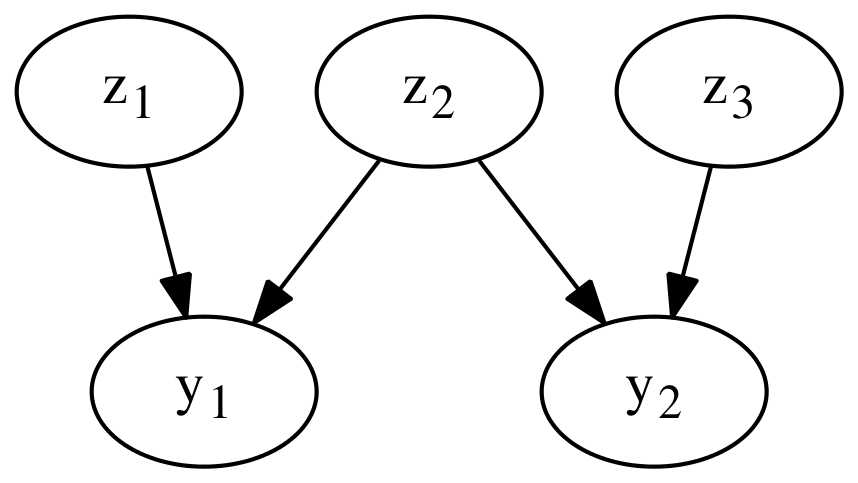
\includegraphics[height=1.2cm]{images/bayesian-network.png}
\end{colfig}

This example can be factorized as follows:
$\text{joint} = p(y_1, y_2, z_1, z_2, z_3) = p(y_1 | z_1, z_2) p(y_2 | z_2, z_3) p(z_1) p(z_2) p(z_3)$

We can then obtain the $z_i$ posterior distribution by marginalizing over the unknown variables:
$p(z_1, z_2, z_3 | y_1, y_2) = \frac{\text{joint}}{p(y_1, y_2)}$\\
$\implies p(z_2 | y_1, y_2) = \sum_{z_1, z_3} \frac{\text{joint}}{p(y_1, y_2)} \propto \underbrace{\sum_{z_1,z_3} \text{joint}}_{\text{message}}$
and to get marginals:
$p(y) = \Pi_i p(y_i)$

$ p(y_i) \overset{\mathclap{\mbox{e.g.}}}{=} \sum_{z_2} p(y_i, z_2) = \sum_{z_2} p(y_i|z_2) \cdot p(z_2)$

\subsection{Belief propagation}
Belief propagation is a message-passing based algorithm used to compute desired marginals (e.g. $p(z_1 | y_1, y_2)$) efficiently. It leverages the factorized expression of the joint. Messages passed:

$m_{z_i \rightarrow y_j}(z_i) = p(z_i) \Pi(\text{messages received by $z_i$ except from } y_j)$, e.g.
$m_{z_1 \rightarrow y_2}(z_1) = p(z_1) m_{y_3\rightarrow z_1}(z_1)
$

$F = \text{set of all variables } y_j \text{ depends upon}$

$ m_{y_j \rightarrow z_i}(z_i) = \sum_{F \neq z_i} p(y_j | F) \Pi_{z \in F\setminus \{z_i\}} m_{z\rightarrow y_j}(z)$, e.g.
$
m_{y_2 \rightarrow z_1}(z_1) = \sum_{z_2} \sum_{z_4} p(y_2|z_1, z_2, z_4) m_{z_2\rightarrow y_2}(z_2)m_{z_4 \rightarrow y_2}(z_4)
$

find a way:
$p(z_i|y_1, y_2) \propto p(z_i) \cdot m_{y_1 \rightarrow z_i} \cdot m_{y_2 \rightarrow z_i}$ (if both exist). Then write messages from definition and write all paths from smallest messages to $z_i$.

% ----------
\section{Kernel}
  Basically, Kernels are a mean to measure distance, or ``similarity'' of two vectors. We define:

  $(\bf{K})_{i,j} = \kappa(\bf{x_i}, \bf{x_j}) = \vec \phi(\bf{x_i})^T \vec \phi(\bf{x_j})$.

  The $\phi$ are not that important in the end, because we only use the Kernel as is. Sometimes it's even impossible to write them down explicitly (RBF).

  \begin{tabular}{ l | l }
    \hline
    Linear     & $\kappa(\bf{x_i}, \bf{x_j}) = \bf{x_i}^T \bf{x_j}$ \\
    \hline
    Polynomial & $\kappa(\bf{x_i}, \bf{x_j}) = (\bf{x_i}^T \bf{x_j} + c)^d$ \\
    \hline
    RBF        & $\kappa(\bf{x_i}, \bf{x_j}) = \exp\left(-\frac{||\bf{x_i} - \bf{x_j}||^2}{2\sigma^2}\right)$ \\
    \hline
  \end{tabular}

  Properties of a Kernel:
\begin{itemize}
\item $\bf{K}$ should be symmetric: $\bf{K}^T = \bf{K}$
\item $\bf{K}$ should be positive semi-definite: $\forall$ nonzero vector $\bf{a}, \bf{a}^T \bf{K} \bf{a} \geq 0$.
\end{itemize}

% -----------
\subsection{Gaussian Process}
The predicting function $f$ is interpreted as a random variable with jointly gaussian prior: $\mathcal{N}(f | \bf{0}, \bf{K})$.
Defining the Kernel matrix $\bf{K} = \kappa(\bf{X}, \bf{X})$ defines the prior. The key idea is, that if $\bf{x}_i$ and $\bf{x_j}$ are
deemed by the kernel to be similar, then we expect the output of $f$ at those points to be similar, too.

We can sample functions from this random variable $f$ and we can use prior + measurements to generate predictions.

If we have measurements $\bf{y}$ available, we get a joint distribution with the $\bf{\hat{y}}$ to be predicted:

$
\begin{bmatrix}
  \bf{y} \\
  \bf{\hat{y}}
\end{bmatrix}
=
\mathcal{N} \left(
  \bf{0},
  \begin{bmatrix}
    \kappa(\bf{X}, \bf{X}) + \sigma_n^2 I  & \kappa(\bf{X}, \bf{\hat{X}}) \\
    \kappa(\bf{\hat{X}}, \bf{X}),          & \kappa(\bf{\hat{X}}, \bf{\hat{X}})
  \end{bmatrix}
\right)
$

This can be marginalized on $\bf{y}$ to find the PDF of $\bf{\hat{y}}$. Advantage: we represent uncertainty.

% ----------
\section{Neural Networks}
A feed forward Neural Network is organized in $K$ layers, each layer with $M^{(k)}$ hidden units $z_i^{(k)}$. Activations $a_i^{(k)}$ are computed as the linear combination of the previous layer's terms, with weights $\bbeta^{(k)}$ (one $(M^{(k-1)} + 1) \times 1$ vector of weights for each of the $M^{(k)}$ activations - $\beta^{(k)}$ size is $M^{(k)} \times (M^{(k-1)} + 1)$ (one for free term, as in linear regression)). Activations are then passed through a (nonlinear) function $h$ to compute the hidden unit $z_i^{(k)}$.

$\bf{x}_n \xrightarrow{\bbeta_i^{(1)}} a_i^{(1)} \xrightarrow{h} z_i^{(1)} \xrightarrow{\bbeta^{(2)}} \dots \xrightarrow{h} \bf{z}^{(K)} = \bf{y}_n$


\subsection{Backpropagation}
Algorithm:
Forward pass: compute $a_i$, $z_i$ and $\bf{y}_n$ from $\bf{x}_n$.
Backward pass: work out derivatives of error to the target $\bbeta_i^{(k)}$ using the chain rule. Emti gives some complicated formulas for that, but regular calculations should work fine.
$\delta^{(k-1)} = \frac{\partial \mathcal{L}}{\partial \bf{a}^{(k-1)}} = diag[ h'(\bf{a}^{(k-1)}) ] \bf{B^{(k)T}} \delta^{(k)}$\\
$\frac{\partial \mathcal{L}}{\partial \bf{B}^{(1)}} = \delta^{(1)} \bf{x}^T$\\
$\frac{\partial \mathcal{L}}{\partial \bf{B}^{(k)}} = \delta^{(k)} \bf{z}^{(k)T}$

\subsection{Regularization}
NN are not \textit{identifiable} (existence of many local optima), so we initialize NN randomly.

NN are universal density estimators (can fit any function), and thus prone to severe overfitting. Techniques used to reduce overfitting include early stopping (stop optimizing when test error starts increasing) and ``weight decay'' (i.e. $L_2$ regularization).

% ----------
\section{Support Vector Machines}
Search for the hyperplane separating the data such that the gap (margin) is biggest.
It minimizes the following cost function (``hinge loss''):

$\mathcal{L}_{SVM} (\bf{\beta})= \sum_{n=1}^N [1 - y_n \tilde\phi_n \beta]_{+} + \frac{\lambda}{2} \sum_{j=1}^M \beta_j^2$

with $[t]_{+} = \max(0, t)$

This is convex but not differentiable. In the dual, the same problem can be formulated as:

$\max_{\alpha \in [0; C]^N} \alpha^T 1 - 1/2 \alpha^T Y K Y \alpha , \alpha^T y = 0$

\section{PCA}
Find the eigenvectors of the covariance matrix $\bf{X^T X}$ of the data. These form an orthonormal basis $\{ \bf{w}_1, ..., \bf{w}_N\}$ for the data in the directions that have highest variance.
One can then use the first $L < D$ vectors to rebuild the data: $\bf{\hat{x}}_i = \bf{W} \bf{z}_i = \bf{W} \bf{W}^T \bf{x}_i$, with $\bf{W} = \begin{bmatrix} \bf{w}_1 ; ... ; \bf{w}_L \end{bmatrix}$.
This minimizes mean square error $\frac{1}{N} \sum_{i=1}^N \bf{x}_i - \bf{\hat{x}}_i^2$.

\section{SVD}
The same as with PCA, we can do with SVD:
\begin{colfig}
  \centering
  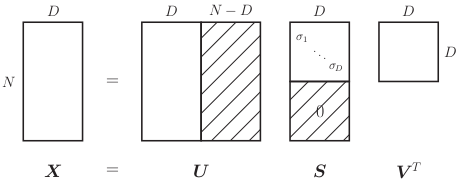
\includegraphics[width=\linewidth]{images/svd.png}
\end{colfig}

The singular vals of a $N \times D$ matrix $\bf{X}$ are the square roots of the eigenvalues of the $D \times D$ matrix $\bf{X^T X}$

\section{Curse of dimensionality}
With the dimensionality increase, every data point becomes arbitrarily far
from every other data point and therefore the choice of nearest neighbor becomes random.
In high dimension, data only covers a tiny fraction of the input space, making generalization extremely difficult.
Or in other words, the volume of the space increases so fast that the available data become sparse.

\section{Primal vs. Dual}
Instead of working in the \textbf{column space} of our data, we can work in the \textbf{row space}:
$$\bf{\hat{y} = X \beta = X X^T \alpha = K \alpha}$$
where $\bf{\beta} \in \mathbb{R}^D$ and $\bf{\alpha} \in \mathbb{R}^N$
and (like magic) $\bf{K}$ shows up, the Kernel Matrix.

Representer Theorem: For any $\bf{\beta}$ minimizing
$$\min_\beta \sum_{n=1}^N \mathcal{L}(y_n, \bf{x}_n^T \bf{\beta}) + \sum_{d=1}^D \lambda \beta_d^2$$
there exists an $\bf{\alpha}$ such that $\bf{\beta = X^T \alpha}$.

When we have an explicit vector formulation of $\beta$, we can use the matrix inversion lemma to get to the dual. E.g. for ridge regression:
$$\beta = (X^T X  + \lambda I_D)^{-1} X^T y = X^T \underbrace{(X X^T + \lambda I_N)^{-1} y}_{\alpha}$$

In optimization, we get to the dual like this:
\begin{colfig}
  \centering
  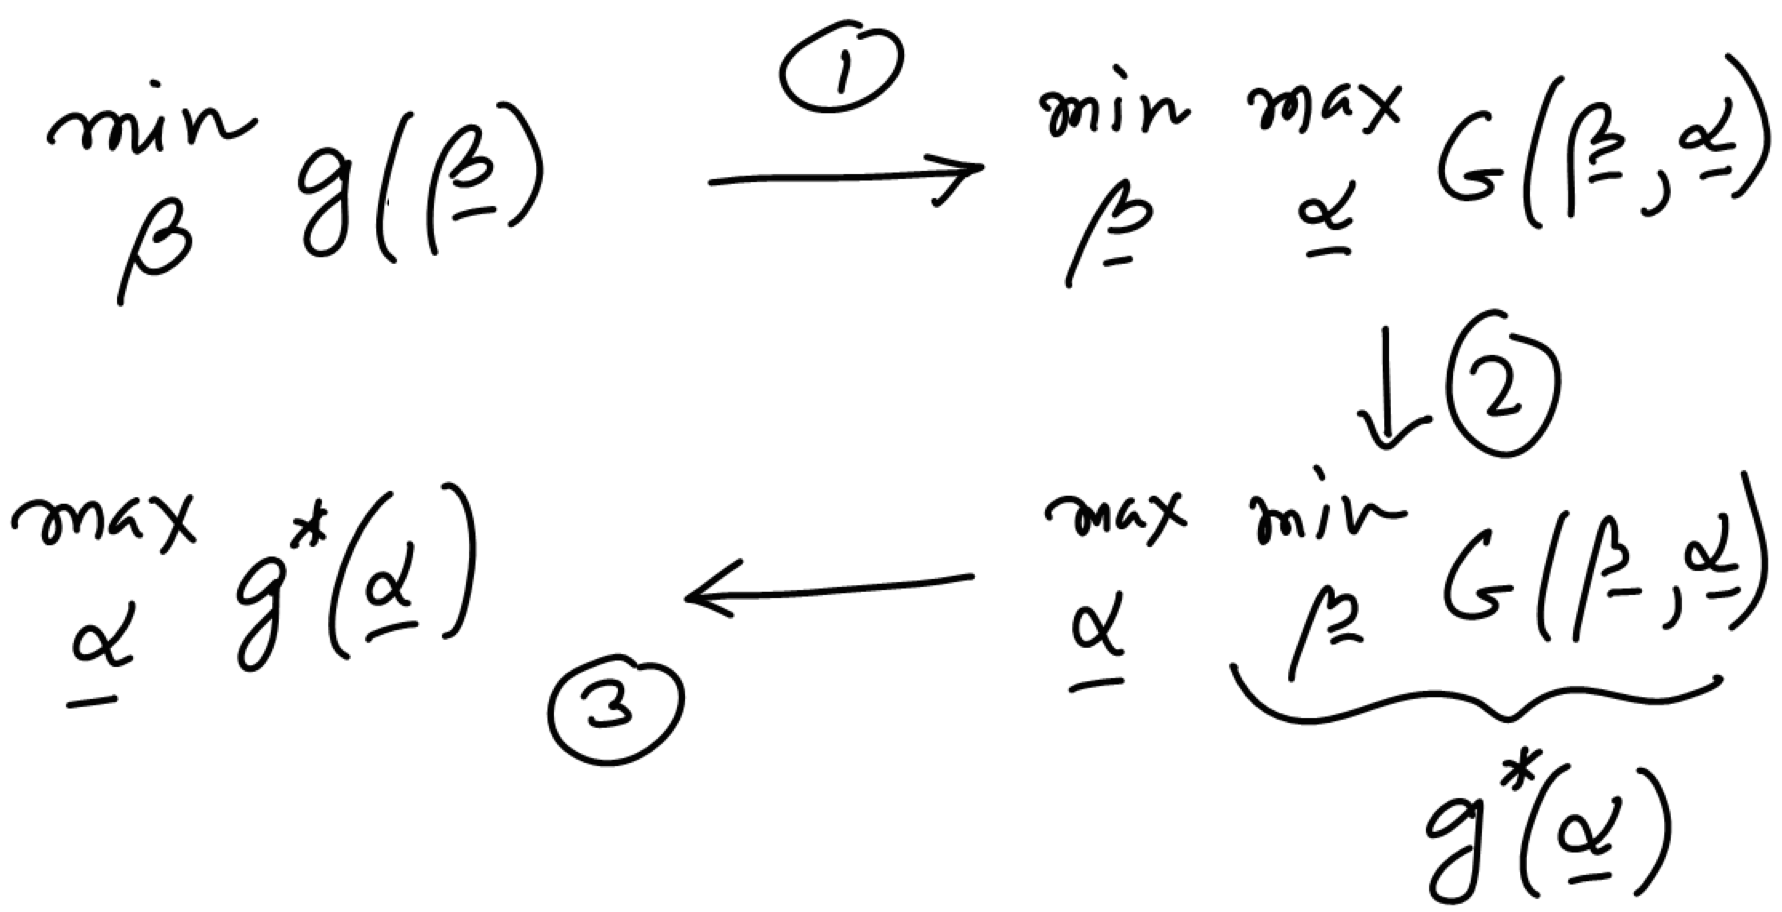
\includegraphics[width=\linewidth]{images/prim-dual.png}
\end{colfig}
% ---------- Footer
\hrule
\tiny
Rendered \today. Written by Dennis Meier, Merlin Nimier-David and Jakub Sygnowski.
\copyright Dennis Meier. This work is licensed under the Creative Commons Attribution-ShareAlike 3.0 Unported License.
To view a copy of this license, visit http://creativecommons.org/licenses/by-sa/3.0/ or
send a letter to Creative Commons, 444 Castro Street, Suite 900, Mountain View, California, 94041, USA.
\includegraphics{images/by-sa.png}

\end{multicols*}
\end{document}
